% DRAFT. Compiles with Tectonic or pdflatex. All numbers are simulation, from analysis/ and data/.
% No participant has been tested. Everything marked TODO needs the team. The earlier five-scheme draft is main_v1_schemes.tex.
\documentclass[conference]{IEEEtran}
\usepackage{amsmath,amssymb,graphicx,booktabs,xcolor}
\usepackage{iftex}\ifPDFTeX\else\usepackage{fontspec}      % Times under XeTeX (Tectonic); pdflatex needs nothing
\setmainfont{texgyretermes}[Extension=.otf,UprightFont=*-regular,BoldFont=*-bold,ItalicFont=*-italic,BoldItalicFont=*-bolditalic]\fi
\newcommand{\todo}[1]{\textcolor{red}{[TODO: #1]}}
\newcommand{\qd}{\dot{q}}
\begin{document}
\title{Seeing the Tilt Limit: A Geofence and Feedback Aid for Teleoperating a Free-Floating Space Arm}
\author{\IEEEauthorblockN{\todo{five names}}\IEEEauthorblockA{MA6223 Human--Robot Interaction, Nanyang Technological University}}
\maketitle

\begin{abstract}
A robot arm on a free-floating spacecraft turns its own base whenever it moves, so a hand target can be
inside the arm's length and still be off limits because reaching it would tilt the spacecraft past its
pointing limit. The operator cannot see that limit. We build a map of it from 98 probe moves in a
momentum-conserving MuJoCo simulation of a 7-joint, 12.5\,kg arm, and wrap the teleoperation in a layered
geofence: three zones on the map with a colour and vibration cue, a hard stop on the target, a simulated
rehearsal of every move, and a runtime fence that brings the hand back if the base passes 2$^\circ$. On
300 targets placed near the edge the map alone is right on 271. With the runtime fence, 46 commands that
a rehearsal refused never took the base past 2.020$^\circ$, and cost a median of 11 to 14\,s each. We
started from the premise that a wrong command is a safety event; the fence shows it is a loss of time, and
we report that as a result. The limit matters only in a band of spacecraft sizes that moves with the
pointing limit: about 150 to 600\,kg at 2$^\circ$, and 600 to 3000\,kg at 0.5$^\circ$. A study of the
feedback with human operators is specified and has not been run.
\end{abstract}

\section{Introduction}
On-orbit servicing puts a human operator in control of an arm whose base is not bolted down. Momentum is
conserved, so every hand motion rotates the spacecraft and moves antennas and sensors off their
targets~\cite{dubowsky1993,umetani1989}. A redundant arm can spend its spare joints on cancelling that
rotation~\cite{nenchev1999,yoshida2001}, but only so far: past a certain reach the base must turn, and how
far the hand gets is then set by how much turn is allowed.

For the operator this creates a boundary in the workspace that nothing marks. A target inside it can be
reached with the base level enough; a target outside it cannot, and the arm either stalls short or tilts
the spacecraft. The boundary depends on direction, on the mass of the spacecraft and on the pointing limit.

\textbf{Problem.} An operator placing hand targets for an arm on a free-floating spacecraft has no view of
the base-tilt limit, so moves are wasted on targets the base cannot afford.

\textbf{Gap.} Reaction null-space work studies what arm motion does to the spacecraft. Virtual
fixtures~\cite{rosenberg1993,abbott2007} and envelope protection are established ways of keeping an operator
inside a boundary. We found no study that fences base tilt for a teleoperated free-floating arm and
measures how well a pre-computed map of that boundary predicts the real one. \todo{Team: read Pietras, Rems
and Walter, IAC-10-B6.2.2, before this paragraph is kept. We have not read it.}

\textbf{Contributions.} (i) A reach map of the tilt limit and its measured error as a detector. (ii) A
layered geofence with graded feedback, and a measurement of what a wrong command costs with it in place.
(iii) The band of spacecraft sizes and pointing limits in which the problem exists. (iv) A negative result:
with a fence, the go or no-go decision is not a safety decision. (v) A study tool for the feedback, ready
to run.

\section{Related Work}
The generalised Jacobian~\cite{umetani1989} gives hand motion of a free-floating arm from joint rates
alone. Reaction null-space control~\cite{nenchev1999} and its flight test on ETS-VII~\cite{yoshida2001}
show zero-reaction manoeuvres, and the loss of reach that comes with them is the dynamic singularity
of~\cite{dubowsky1993}. Null-space impedance toward a rest posture keeps the arm's shape repeatable for the
operator~\cite{hogan1985,dragan2013}. Virtual fixtures~\cite{rosenberg1993,abbott2007} constrain or guide
the operator's commands in telemanipulation; our hard stop on the target is a forbidden-region fixture
whose region is defined by base tilt instead of by geometry. In the work we have read, the reach left by
a limit on base tilt is a result for the controller; it is not shown to the operator before the command.

\section{Model and Controller}
The system is a rigid base on a free joint with a 7-revolute arm (z-y-z-y-z-y-z, reach 1.09\,m, 12.5\,kg),
no gravity and no contact, simulated in MuJoCo~\cite{todorov2012} and controlled at 100\,Hz. Three base
masses are modelled: 30, 300 and 3000\,kg. With base twist $v_b$ and joint rates $\qd$,
\begin{equation}
H_b v_b + H_{bm}\qd = 0 ,\qquad \dot{x} = (J_m + J_b V)\,\qd = J^{*}\qd ,
\end{equation}
with $V=-H_b^{-1}H_{bm}$ when starting from rest. Let $W$ be the three angular rows of $V$; the base does
not rotate exactly when $W\qd=0$. Under random joint commands for 10\,s the base-row momentum stays below
$10^{-6}$ in SI units, and $J^{*}\qd$ and $W\qd$ match the simulated hand and base velocities to $10^{-6}$.

The controller tracks a hand position target with the task and the reactionless condition solved
together, and a pull toward a rest posture in the freedom that is left (null-space impedance plus
reaction null space). The hand rows are weighted 2 to 1 against the base rows. The weight changes nothing while the arm can
satisfy both; when it cannot, the hand keeps its path and the base takes the rest. Joints
are held inside their ranges by locking a joint that is within 0.05\,rad of its limit and still commanded
outward. Five redundancy schemes were compared before this one was chosen; on the 300\,kg spacecraft the
reactionless schemes cut peak base drift sixfold on a position-only path (0.20$^\circ$ against
1.22$^\circ$) with tracking under 0.2\,mm. \todo{Cite the earlier draft as a report or move its Table I to
an appendix if pages allow.}

\textbf{Why reach is bought with tilt.} Restricted to joint motions that do not turn the base, the hand
Jacobian of the 300\,kg spacecraft at rest has singular values 0.36, 0.10 and 0.08, against 0.22 to 0.74
unrestricted. One direction stays about four times freer than the other two. Over 6000
random postures the smallest value never exceeds 0.10, so no starting posture removes the limit. The tilt
does not fully come back with the hand: after 0.3\,m out and back the base is still 0.30$^\circ$ off and the
joints are 1.24\,rad from where they started. From the earlier rest pose this was 0.00$^\circ$, so it depends on the pose.

\section{The Reach Map}
From the rest posture the hand is pulled along 98 directions (the distinct directions of a
$5\times5\times5$ integer grid). On each line we record how far the hand gets before the base has tilted
0.5$^\circ$, 1$^\circ$ and 2$^\circ$. The three sets of 98 points are joined into three nested surfaces, drawn
in the operator's view as cages around the hand.

The \emph{depth} of a target is its distance from the rest position divided by the distance to the
2$^\circ$ surface along the same line: 0 at rest, 1 on the surface.

A \emph{rehearsal} is a simulated copy of the commanded straight move from the current state. It reports
the target reachable if the hand arrives within tolerance before the base passes 2$^\circ$ and before the hand
stalls. We use the rehearsal as the reference the map is scored against; its own error is measured in
Section~\ref{sec:fence}.

\section{Geofence and Feedback}
Safety is given to the fence and the display is left to save the operator time. The layers, from earliest
warning to last stop:
\begin{enumerate}
\item \textbf{Zones.} Depth under 0.90 is free, 0.90 to 1.10 is caution, above 1.10 is closed. The two
thresholds are where the map stops being reliable (Section~\ref{sec:map}).
\item \textbf{Graded cue.} The target marker is green in the free zone and yellow in the caution zone; it
turns red when a rehearsal refuses the target. On a gamepad the vibration rises linearly from zero at depth
0.90 to full at 1.10. \todo{Vibration is written and has never been run on a controller.}
\item \textbf{Hard stop on the target.} The target cannot be pushed past depth 1.10; it slides along that
surface.
\item \textbf{Rehearsal gate.} Each command is rehearsed and refused if the rehearsal fails.
\item \textbf{Runtime tilt fence.} If the real base still passes 2$^\circ$ during a move, or the move
exceeds a time limit, the hand is sent back to where the move started.
\item \textbf{Joint limits}, as above.
\end{enumerate}
Layers 1 to 3 act while the operator is still choosing; 4 acts at the command; 5 and 6 act during the move.
Fig.~\ref{fig:opview} shows what the operator sees. The map is probed from rest, and from another start it
is less right: after a 0.3\,m detour of the hand the rehearsal changed its answer on 5 of 100 goals at 0.8 of
the edge and on 24 of 100 at the edge. So the cages are a guide, and the rehearsal, which runs from the true
state, decides.
\begin{figure}[t]\centering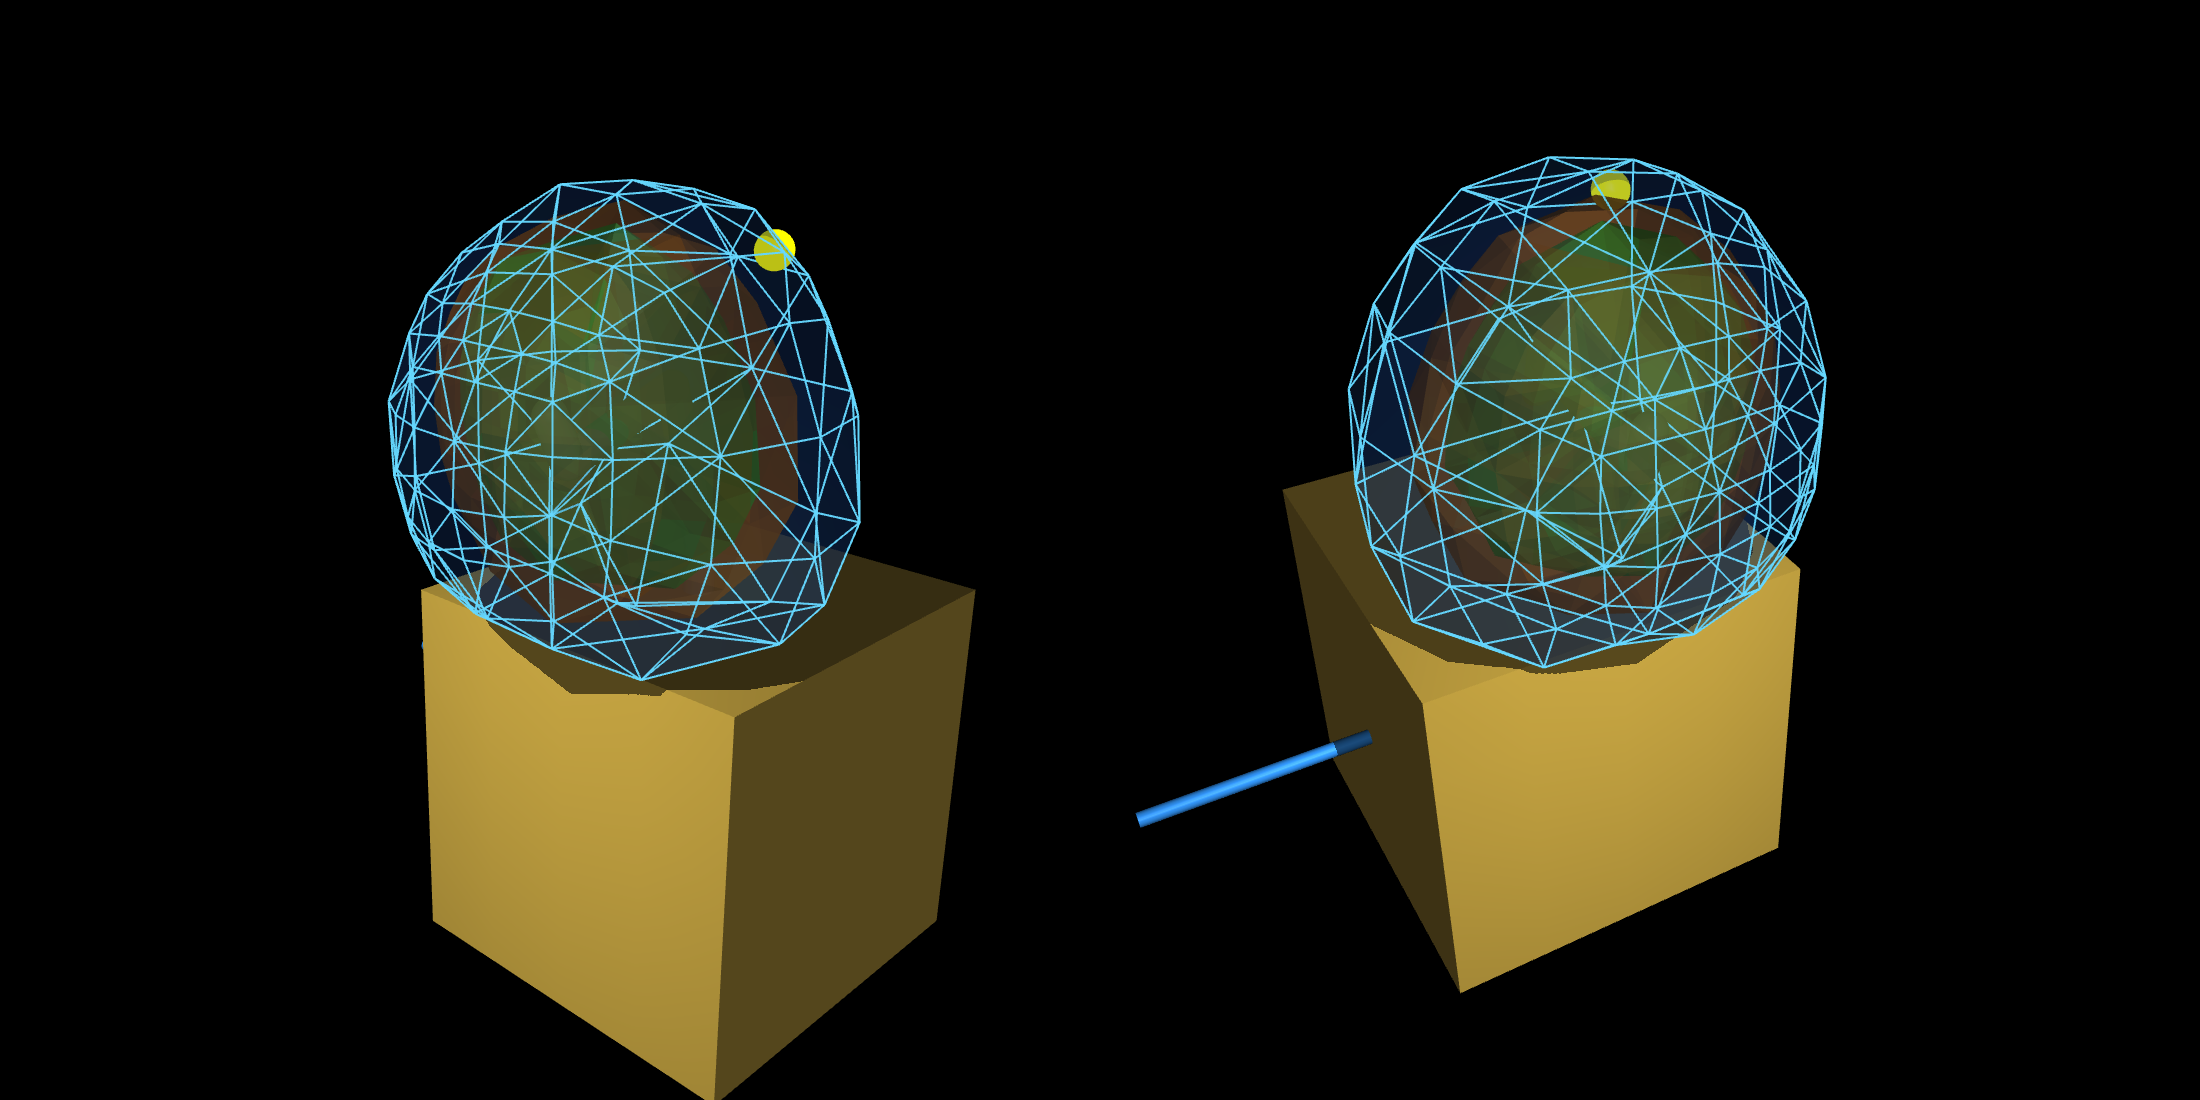
\includegraphics[width=\columnwidth]{figs/fig_opview}
\caption{Operator view, two camera angles, 300\,kg spacecraft with the arm at rest inside the cages. Blue cage:
base tilt reaches 2$^\circ$. Orange and green volumes: 1$^\circ$ and 0.5$^\circ$. Yellow dot: a target at
depth 1.0, in the caution zone. Rendered offscreen with the viewer's drawing code.}\label{fig:opview}\end{figure}

\section{Results}
All results are from simulation. The 300\,kg spacecraft is used unless stated.

\subsection{The map as a detector}\label{sec:map}
We placed 300 targets at depths 0.75 to 1.25 and rehearsed each; 162 were reachable. Calling a target
reachable when its depth is under 1, the 98-line map is right on 271, says go for 8 that fail and no-go
for 21 that work (Table~\ref{tab:map}). A 26-line map is right on 229. Moving the threshold trades one error
for the other: at 0.85, 1 false go and 100 false no-go; at 1.10, 54 and none. No single threshold is safe
and useful at once, which is the reason for three zones: of 89 targets under depth 0.90, 86 are reachable;
of 84 above 1.10, none; of the 127 between, 76.

\begin{table}[t]
\caption{Map against rehearsal, 300 targets near the edge}\label{tab:map}
\centering\begin{tabular}{lccc}\toprule
Rule & False go & False no-go & Right\\\midrule
98 lines, depth $<1$ & 8 & 21 & 271\\
26 lines, depth $<1$ & 13 & 58 & 229\\
98 lines, depth $<0.85$ & 1 & 100 & 199\\
98 lines, depth $<1.10$ & 54 & 0 & 246\\\bottomrule
\end{tabular}\end{table}

\subsection{Wrong mass}
The map is built for one spacecraft mass. With the true mass 10\% lower, equal and 10\% higher, on 120
targets, the nominal map gives 4, 1 and 1 false go and 4, 6 and 10 false no-go. One of the 98 directions
changes reach by more than 30\%. The effect is real and small, and we do not make it a headline.

\subsection{What a wrong command costs}\label{sec:fence}
To test the last layer alone we switched the rehearsal gate off and commanded 46 targets that a rehearsal
had refused (Table~\ref{tab:fence}).
% FENCE-TABLE-BEGIN (numbers from analysis/envelope/fence.py)
\begin{table}[t]
\caption{Runtime fence on 46 commands that a rehearsal refused}\label{tab:fence}
\centering\begin{tabular}{lcccc}\toprule
Outcome & $n$ & Peak tilt & Tilt left & Time\\\midrule
Tilt trip & 33 & 2.020$^\circ$ & 0.12$^\circ$ & 14 (19)\,s\\
Stall & 10 & 1.76$^\circ$ & 0.04$^\circ$ & 11 (14)\,s\\
Time limit & 1 & 1.53$^\circ$ & 0.00$^\circ$ & 18\,s\\
Arrived & 2 & 1.93$^\circ$ & 1.93$^\circ$ & 7 (8)\,s\\\bottomrule
\multicolumn{5}{l}{\footnotesize Tilt: worst case. Time: median (worst), out and home.}
\end{tabular}\end{table}
% FENCE-TABLE-END
The time limit is 13.1\,s, 1.5 times the slowest of 41 reachable moves from rest (median 4.8\,s, slowest
8.8\,s). The base never passed 2.020$^\circ$. 44 of the 46 ended with the hand home and the base within
0.12$^\circ$ of level, the worst after 19\,s. A wrong command therefore costs time, a median of 11 to 14\,s
depending on how it ends, and not attitude. The study tool charges 8\,s for a rehearsal; that is a set value, not a measurement.
Two weaknesses remain. The other 2 of the 46 arrived inside 8\,s with the base at 1.2 and 1.9$^\circ$: the
rehearsal we score the map against refuses a target the arm reaches, about once in 23. And the fence bounds
tilt but does not promise a level base afterwards: 0.12$^\circ$ was the most left here, and a plain 0.3\,m
move out and back leaves 0.30$^\circ$.

\subsection{Where the problem exists}
\begin{figure}[t]\centering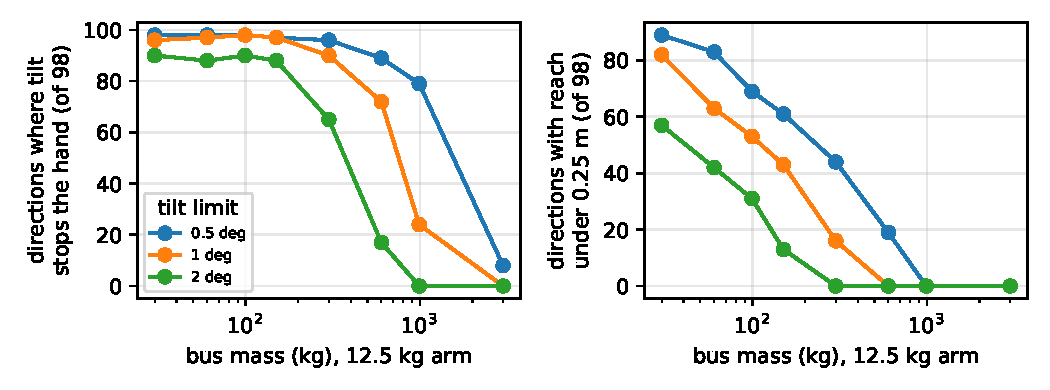
\includegraphics[width=\columnwidth]{figs/fig_band}
\caption{Left: number of the 98 directions in which base tilt, not arm length, stops the hand. Right: number
in which reach is under an assumed parking error of 0.25\,m. The aid is useful where the left curve is high
and the right curve is low.}\label{fig:band}\end{figure}
We scaled the base mass and inertia of the 300\,kg model from 30 to 3000\,kg and rebuilt the map at each of
eight masses (Fig.~\ref{fig:band}). On a heavy spacecraft tilt never binds: at 3000\,kg and 2$^\circ$ no
direction is limited by tilt, and the map is just the arm's length. On a light one the usable reach is
smaller than any plausible parking error: at 30\,kg and 2$^\circ$, 53 of 98 directions give under 0.25\,m.
Between them is a band where tilt binds and useful reach remains: about 150 to 600\,kg at 2$^\circ$, with
81, 63 and 33 directions bound at 150, 300 and 600\,kg. Tightening the limit moves the band up: at
0.5$^\circ$, 600\,kg still has 96 directions bound by tilt and 3000\,kg has 15. \todo{The 0.25\,m parking error is an assumption with no source. Find one or
plot several values.} Inertia was scaled in proportion to mass, which is cruder than a real bus, so the
edges of the band are approximate.

\section{Operator Study}
\todo{Not run. No participant data exists, and none may be invented.} The study tool presents targets near
the edge and records every command, refusal and time. Planned design: within-subject, three conditions in
shuffled order: no cue (cages hidden), colour cue, colour cue plus hard stop. The runtime fence is on in
all three. Measures: time per target reached, number of refused or aborted commands, peak base tilt, and
NASA-TLX~\cite{hart1988} after each condition. Hypothesis: the colour cue reduces refused and aborted
commands and time per target, and the hard stop reduces them further. The tool scores each
target in seconds: the time to reach it, plus 30\,s when the operator gives it up as out of reach. The 30\,s
is a set value. Every send starts from rest, as the map
was probed: a second send on the same target first puts the arm back at rest, at no cost in time. \todo{Ethics statement, statistics.}

\section{Discussion}
\textbf{A premise that failed.} We began by treating the go or no-go decision as the operator's risky
choice, and scored a failed command twenty times worse than a rehearsal. Section~\ref{sec:fence} removes
the ground for that: once a runtime fence exists, a failed command is a detour. The operator's problem is
then one of efficiency, and the safety property belongs to the fence, where it can be tested without a
human.

\textbf{What the human is for.} The fence and the rehearsal can refuse a target but cannot choose one. The
display tells the operator which targets are cheap, which are uncertain and which are closed before any
command is sent.

\textbf{Attitude control.} We model a spacecraft with no attitude control during arm motion.
\todo{Unchecked: we believe most servicers keep attitude control on. Find a source.} If the base is held
with reaction wheels the quantity to fence is the momentum the wheels must absorb, which for this arm is
$h=Kv$ with $K$ between 8 and 11\,kg\,m at rest across nine base masses, about 0.8 to 1.1\,N\,m\,s at
0.1\,m/s. It scales with the arm and the hand speed and not with the spacecraft. The same layers apply
with that quantity in place of tilt; we have not built that version.

\textbf{Limitations.} Simulation only; no participants. One arm, one rest posture, maps built from rest.
No contact, flexible appendages, joint friction, sensor noise or initial momentum. The reference
(rehearsal) has a measured error of its own. The fence does not guarantee a level base after a stall. The
time limit comes from one spacecraft size. Zone thresholds were read off 300 targets on one spacecraft and
not re-tested on fresh targets.

\section{Conclusion}
The tilt limit of a free-floating arm can be drawn for the operator from 98 probe moves and is right on
271 of 300 targets near its edge. A layered geofence holds the base at its limit whatever is commanded,
and turns a wrong command from a hazard into a delay of 11 to 14\,s. The problem is confined to a band of
spacecraft sizes that depends on the pointing limit. Whether the feedback helps people is not yet known.

\bibliographystyle{IEEEtran}
% TODO: check every entry against P2_Literature_Survey.xlsx; these were written from memory.
\begin{thebibliography}{99}
\bibitem{dubowsky1993} S. Dubowsky and E. Papadopoulos, ``The kinematics, dynamics, and control of free-flying and free-floating space robotic systems,'' \emph{IEEE Trans. Robot. Autom.}, vol. 9, no. 5, 1993.
\bibitem{umetani1989} Y. Umetani and K. Yoshida, ``Resolved motion rate control of space manipulators with generalized Jacobian matrix,'' \emph{IEEE Trans. Robot. Autom.}, vol. 5, no. 3, 1989.
\bibitem{nenchev1999} D. N. Nenchev, K. Yoshida, P. Vichitkulsawat, and M. Uchiyama, ``Reaction null-space control of flexible structure mounted manipulator systems,'' \emph{IEEE Trans. Robot. Autom.}, vol. 15, no. 6, 1999.
\bibitem{yoshida2001} K. Yoshida, K. Hashizume, and S. Abiko, ``Zero reaction maneuver: flight validation with ETS-VII space robot and extension to kinematically redundant arm,'' in \emph{Proc. IEEE ICRA}, 2001.
\bibitem{hogan1985} N. Hogan, ``Impedance control: an approach to manipulation,'' \emph{ASME J. Dyn. Syst. Meas. Control}, vol. 107, 1985.
\bibitem{dragan2013} A. D. Dragan, K. C. T. Lee, and S. S. Srinivasa, ``Legibility and predictability of robot motion,'' in \emph{Proc. ACM/IEEE HRI}, 2013.
\bibitem{rosenberg1993} L. B. Rosenberg, ``Virtual fixtures: perceptual tools for telerobotic manipulation,'' in \emph{Proc. IEEE Virtual Reality Annu. Int. Symp.}, 1993.
\bibitem{abbott2007} J. J. Abbott, P. Marayong, and A. M. Okamura, ``Haptic virtual fixtures for robot-assisted manipulation,'' in \emph{Robotics Research}, Springer, 2007.
\bibitem{todorov2012} E. Todorov, T. Erez, and Y. Tassa, ``MuJoCo: a physics engine for model-based control,'' in \emph{Proc. IEEE/RSJ IROS}, 2012.
\bibitem{hart1988} S. G. Hart and L. E. Staveland, ``Development of NASA-TLX: results of empirical and theoretical research,'' in \emph{Human Mental Workload}, 1988.
\end{thebibliography}
\end{document}
